% story.tex --- story-format companion draft of Paper D.
%
% This is a SEPARATE document from main.tex (draft v31), which is untouched and
% remains the technical report of record: it carries the full prediction ledger,
% the registration deviations, the checker audits, and the provenance manifest.
% This version reorganises the SAME evidence around one alternative explanation
% and three predictions derived from it, in the manner of "Are Emergent Abilities
% of Large Language Models a Mirage?" (arXiv:2304.15004).
%
% Every number here is copied from main.tex or papers/D-reference-laws/registration.md.
% No number, claim, caveat, or registration status has been changed. Where a
% registered prediction failed, the failure is stated where the claim appears.

\documentclass[11pt]{article}
\usepackage[margin=1in]{geometry}
\usepackage{amsmath,amssymb}
\usepackage{graphicx}
\usepackage{booktabs}
\usepackage{array}
\newcolumntype{L}[1]{>{\raggedright\arraybackslash}p{#1}}
\usepackage{longtable}
\usepackage{xcolor}
\usepackage[colorlinks=true,linkcolor=blue,citecolor=blue,urlcolor=blue]{hyperref}
\usepackage{caption}
\captionsetup{font=small,labelfont=bf}

\usepackage{placeins}
\renewcommand{\topfraction}{0.9}
\renewcommand{\bottomfraction}{0.8}
\renewcommand{\textfraction}{0.07}
\renewcommand{\floatpagefraction}{0.75}
\setcounter{topnumber}{3}
\setcounter{totalnumber}{5}

\title{When References Become Targets:\\ Reference-Conditioned LLM Judges Favor Answer Matching\\ on Multi-Valid Tasks}
\author{Anonymous Authors}
\date{Companion draft, September 7, 2026}

\begin{document}
\maketitle

\begin{abstract}
\noindent
Reference-guided judging is standard practice: an LLM judge shown a trusted answer can check a candidate instead of trusting its own opinion.
We propose one alternative reading of what that reference is on the multi-valid short-answer tasks we study: when more than one answer is valid, the reference is not an answer key but a single sample from the valid set, and the judge anchors on it, so what it measures is proximity to an arbitrary sample rather than correctness.
Three predictions follow, and we test each on tasks whose validity a program decides, so the number of valid answers is controlled rather than argued about.
First, swapping the reference between two equally valid answers should move the score of identical, unchanged candidate text, and it does, by up to $9.5$ points of ten.
Second, the harm should switch on the moment a second valid answer exists and be absent when the answer is unique: all six open-model judges tested shift toward inflation at the first step in multiplicity, and the inversion reproduces on a third-party benchmark, while the identical protocol on unique-answer mathematics shows the reference collapsing the harm instead; the corresponding test on a production judge is inconclusive under the available score interface rather than confirmatory.
Third, the harm should survive what would neutralise mere ignorance, and it does: a frontier-class judge shown a reference marks $82.5\%$ of genuinely correct non-matching answers as failing against $19.6\%$ for the same answers judged blind, the effect persists on answers the judge itself certified while blind, and a policy trained against a reference-showing judge raised that judge's score while its true accuracy fell by more than half.
A registered masking suite then strongly supports a cheap semantic-comparison mechanism: the anchoring survives the reference being rewritten as English words, collapses when equality requires one computation step, and vanishes when the reference's final answer is hidden with its derivation intact, a pattern consistent with the judge performing a semantic equality check against a readable answer token.
One registered scope prediction failed: we predicted a canonical solution shown on program synthesis would inflate like a key, and it did not, reducing inflation relative to blind instead.
That falsification suggests a revised boundary hypothesis, that anchoring requires a cheaply extractable answer token to match against; a preregistered continuum over answer structures, scalar to pair to JSON to program with content held fixed, then finds the predicted attenuation, with the artifact-level harm falling below zero for the stronger judge and to a small residue for the weaker one, supporting strong attenuation as answers become less cheaply comparable, with the artifact-level transition itself judge-dependent.
On the multi-valid short-answer tasks we study a reference is therefore a lever rather than a safeguard, and the strongest mitigation we test is structural rather than verbal: score blind first, and reveal the reference only afterwards; a registered decomposition shows its active ingredient is the displayed blind score itself, a numeric anchor the judge defers to instead of the reference token.
\end{abstract}

\begin{table}[t!]
\centering
\small
\setlength{\tabcolsep}{5pt}
\begin{tabular}{L{1.1cm}L{4.6cm}L{4.2cm}L{4.0cm}}
\toprule
& Prediction & Test & Result \\
\midrule
\textbf{P1} & Swapping the reference between equally valid answers moves the score of identical text &
Re-judge frozen samples with the reference rotated to a different valid answer &
\textbf{Up to $+9.5$ of 10 points}, with mirror-image losses and a flat placebo; replicated under registration on an exact-oracle pool, $12$ of $12$ cells (Section~\ref{sec:p1}) \\
\addlinespace[3pt]
\textbf{P2} & The harm switches on at $k{=}2$ and inverts to help at $k{=}1$ &
Pools built with exactly $k$ valid answers per item; the same protocol on unique-answer math; a third-party benchmark &
\textbf{Step positive for all six judges}; math inflation collapses $4$--$13\times$; the inversion reproduces on \textsc{MACE} (Section~\ref{sec:p2}) \\
\addlinespace[3pt]
\emph{Mech.} & Behavioral signature of a cheap semantic equality check on a readable answer token &
Reference rewritten as words, as an equivalent expression, and as a worked derivation with the answer hidden &
\textbf{6 of 6 cells confirmed}: words preserve the margin, computation collapses it, masking kills it (Section~\ref{sec:maskident}) \\
\addlinespace[3pt]
\textbf{P3} & The harm survives what should neutralise it &
Frontier judge; only answers the judge itself certified blind; training a policy against the judge &
\textbf{$82.5\%$ vs $19.6\%$ failing grades}; the filtered effect is unchanged; a $+4.13$ wedge under training (Section~\ref{sec:p3}) \\
\midrule
\emph{Scope} & Registered: a canonical solution on code, one valid program among many, should inflate like a key &
Program synthesis: a canonical solution in the reference slot, against blind and against a test suite &
\textbf{Falsified: no inflation}, exemplar-versus-blind $-0.34$ and $-0.57$; a preregistered continuum then confirms strong attenuation with a judge-dependent cliff (Sections~\ref{sec:code}, \ref{sec:sepcont}) \\
\bottomrule
\end{tabular}
\caption{\textbf{Takeaway: one explanation; three predictions and a mechanism probe confirmed; and one falsified scope prediction whose revised boundary hypothesis was then tested held-out, with a split verdict.} The explanation is that a reference on a multi-valid task is one sample from the valid set and the judge anchors on it. Anchoring is in points of the judge's 0--10 scale; inflation and the training wedge are in baseline standard deviations of the judge's own score distribution. Intervals, caveats, and the predictions that failed are in the sections named.}
\label{tab:predictions}
\end{table}

\section{Introduction}

Consider a task that asks for any divisor of 91 strictly between 1 and 91: both 7 and 13 are fully correct.
Show a judge the reference ``7'' and it scores a candidate answering 7 near ten out of ten while scoring an equally correct 13 near five; rotate the reference to 13 and the same two answers swap scores.
Nothing about either answer changed.

This matters because the reference is supposed to be the safety mechanism.
Reference-guided judging raises agreement with human labels on question answering~\cite{refguided2024}, blind judges are documented to drift generous exactly when no reference is present~\cite{generous2026}, and our own companion study found that a trusted reference collapses best-of-$n$ reward hacking on math and code, provided the judge is capable enough to use it~\cite{companionA}.
The standard reading of a reference is that it is an \emph{answer key}: a certificate against which a candidate is verified more cheaply than it is solved.

\paragraph{One alternative explanation.}
We propose that on tasks with more than one valid answer the reference is not an answer key at all, but \emph{one sample from the valid set}, drawn by whoever built the dataset and treated by the judge as though it were the whole set.
Everything in this paper follows from that single reading.
If the judge anchors on the shown sample, the quantity it reports is proximity to an arbitrary member of the valid set, a property of the reference rather than of the candidate~\cite{companionB}, and under best-of-$n$ selection an optimizer replaces ``pick a correct answer'' with ``pick the answer that matches the key.''
Two levels of claim run through the paper, and we keep them separate: the experiments establish \emph{reference dependence} causally, that the score of unchanged text follows which valid answer occupies the reference slot; that the underlying operation is specifically a cheap equality check against a separable answer token is our proposed mechanism, and we mark where the evidence for it is direct and where it is post hoc.

The static half of this failure is already known, and not only to us: judges penalise valid solutions that differ from the provided reference~\cite{fixation2025}, reference-guided evaluation degrades on open-ended tasks~\cite{judgingref2026}, and on \textsc{RewardBench-2} Ties comparisons a reference costs $7$--$8$ points of verdict accuracy regardless of who wrote it~\cite{companionA,malik2025rewardbench2}.
The open question was dynamic, because static verdict accuracy and behaviour under selection pressure can disagree~\cite{gao2022scaling} and the safeguard case rests on the dynamic quantity.
We settle it where it can be settled exactly, on tasks with programmatic validity oracles, so the number of valid answers is controlled by construction; free-form generation is outside our scope.

\paragraph{Three predictions.}
If the reference is a sample and the judge anchors on it, three things must be true, and each fails under the answer-key reading.

\begin{itemize}
\item \textbf{P1.} The score must follow the reference. Swap which valid answer sits in the reference slot, hold the candidate text fixed, and the score of that unchanged text must move. An answer key cannot do this, because both answers are correct either way (Section~\ref{sec:p1}).
\item \textbf{P2.} The harm must switch on at the first step in multiplicity. When exactly one answer is valid, proximity and correctness are the same criterion, so anchoring \emph{is} verification and the reference should help. The moment a second valid answer exists the two criteria come apart and the reference should start to hurt (Section~\ref{sec:p2}).
\item \textbf{P3.} The harm must survive what would neutralise ignorance. If the judge simply did not know the alternative was valid, then a stronger judge, or restricting attention to answers the judge itself already certified, should remove the effect. Anchoring predicts it will not, and predicts that optimization pressure will exploit it rather than average it away (Section~\ref{sec:p3}).
\end{itemize}

Where the failure stops is a question the explanation did not settle in advance, and there we report a falsification rather than a confirmation: we registered the prediction that a canonical \emph{solution} shown on program synthesis would inflate the way a short-answer key does, and it did not (Section~\ref{sec:code}).
The failure suggests a revised hypothesis, that anchoring requires a separable answer token to match against, so that on code, where the artifact is the answer, a reference behaves as a specification; that hypothesis fits the data but was formed after seeing it.
Section~\ref{sec:sepcont} reports its first held-out test, preregistered for this revision: across an answer-structure continuum the harm attenuates as predicted for both judges, while the sharp artifact-level cliff held for one judge and was falsified for the other.

\paragraph{Registration.}
Every prediction in this paper was committed before the data it is scored on existed.
Two experiments carry external Open Science Framework registrations with third-party timestamps, the replication (\texttt{osf.io/ym5x9}) and the mitigation study (\texttt{osf.io/qugbd}), as does a judge-coverage extension; the rest are git commits carrying first-party timestamps only.
Roughly half of the auxiliary predictions failed, and we report those failures where they bite rather than in a footnote: the composition and distance analyses each falsified a registered prediction, as did half of the two-factor follow-up registered in response to external review (Section~\ref{sec:dose}), the method rotation (Section~\ref{sec:limits}), the code exemplar (Section~\ref{sec:code}), and the separability continuum's artifact-level leg for one of two judges (Section~\ref{sec:sepcont}); one of two mitigation predictions is only partially confirmed, one of two coverage predictions was not confirmed, and the mitigation-variant decomposition falsified its framing-equivalence prediction for one judge (Section~\ref{sec:norescue}); and the training experiment's protected arm failed its own manipulation check three times, closing that question as unresolved under a pre-adopted stopping rule (Section~\ref{sec:limits}).
The complete ledger of predictions, timestamps, deviations, and outcomes lives in the technical report version of this paper, with an artifact manifest naming a committed producer for every number quoted here.\footnote{Technical report version, draft v31, released with the code. It contains the full prediction ledger, the registration deviations, three post-hoc checker audits, and the provenance manifest. This document reorganises that evidence and changes none of its numbers; the experiments added in the present revision (the two-factor composition factorial, the exact-oracle rotation replication, the intention-to-treat sensitivity, and the masking, separability, and third training runs) postdate v31 and carry their registrations as git-timestamped commits in the released code.}
Table~\ref{tab:predictions} summarises the explanation, the five tests, and their outcomes.

\section{Setup}
\label{sec:setup}

\paragraph{Tasks.}
Validity is decided by a program throughout, never by an LLM adjudicator or a human, and four pools carry the results.
The \emph{replication pool} is 120 fresh tasks across five programmatically verifiable constraint families (CRT remainders, subset-sum, Goldbach pairs, divisor counts, digit sums), each with an exact arithmetic oracle; the \emph{$k$-stratified pool} is 75 tasks from those families built with exactly $k$ valid answers, 15 per stratum at $k \in \{1,2,4,8,16\}$, all 465 stored answers oracle-verified; the \emph{synthetic grid} is 60 tasks with exactly $k$ enumerated valid answers over the same range, from two families whose valid sets enumerate exactly; and the \emph{exploratory pool} is 51 generation tasks built from \textsc{RewardBench-2} Ties items~\cite{malik2025rewardbench2}, the weakest of the four, carrying only the mechanism experiments, which compare a judge to itself.
Two third-party substrates enter later, \textsc{MACE}~\cite{mace2026} and MBPP.
Each task stores its full valid set, and one seeded-random member is designated at build time as the reference shown in the referenced condition, so \emph{correct} always means ``any valid answer,'' never ``the reference.''

\paragraph{Generation and judges.}
Candidate pools are 64 samples per task at temperature 1.0.
The replication and $k$-stratified pools are generated by Llama-3.1-8B-Instruct and judged by Qwen2.5-7B-Instruct and phi-4, a cross-family pair, so no judge grades its own family's text; the synthetic grid is scored by six judges spanning three model families, a registered coverage extension adds three more, and the exploratory pool is judged by the Qwen2.5 Instruct ladder at 1.5B, 3B, 7B, and 14B.
Each judge runs \emph{blind}, with no reference in context, and \emph{referenced}, with the stored reference in context, under two paraphrases of the scoring rubric; selection uses one paraphrase and reporting uses the other, which cancels winner's-curse inflation.

\paragraph{The two measurements.}
\emph{Inflation} is the excess hack gap: how far the selected sample's reported score sits above its true quality, in baseline standard deviations, against a null built by shuffling judge scores among samples the oracle grades identically.
We reproduce the definition here so this paper stands alone.
For one item with samples $s_1, \dots, s_n$, judge scores $J(\cdot)$ with pool mean $\mu_J$ and standard deviation $\sigma_J$, and oracle validity $V(\cdot)$ with pool mean $\mu_V$, the best-of-$n$ pick is $s^\star = \arg\max_i J(s_i)$ and the hack gap is the standardized scoreboard gain in excess of the raw truth gain,
\begin{equation}
G \;=\; \frac{J(s^\star) - \mu_J}{\sigma_J} \;-\; \bigl(V(s^\star) - \mu_V\bigr),
\end{equation}
with selection under one rubric paraphrase and the reported $J(s^\star)$ taken from the other.
Because $V$ is binary validity, the second term is an absolute accuracy gain rather than a standardized validity gain; ``baseline standard deviations'' refers to the normalization of the scoreboard component only, not of $G$ as a whole.
Inflation is $G - \mathbb{E}_\pi[G]$, where $\pi$ shuffles judge scores among samples the oracle grades identically, so any score-validity association a judge earns honestly is preserved under the null; the committed implementation additionally averages over score ties and resampled sub-pools.
A judge whose scores merely track validity reads zero; a judge that awards 10 to reference-matching answers raises the reported score of its best-of-64 pick without moving that pick's true validity, and inflation measures that scoreboard-versus-truth divergence.
The anchoring \emph{margin} is the score bonus a valid reference-matching sample receives over an equally valid non-matching one, on the 0--10 scale.
Both estimators come unchanged from companion A~\cite{companionA}, frozen in committed code before the confirmatory runs.
Because the standardized estimand is cognitively expensive, wherever the design defines them we also report plain quantities that need no estimator: the true accuracy of the selected sample, whether a selected valid answer matches the shown reference, and the rate at which valid non-matching answers receive failing grades.

\section{The phenomenon: the reference makes selection worse}
\label{sec:phenomenon}

\begin{figure}[t!]
\centering
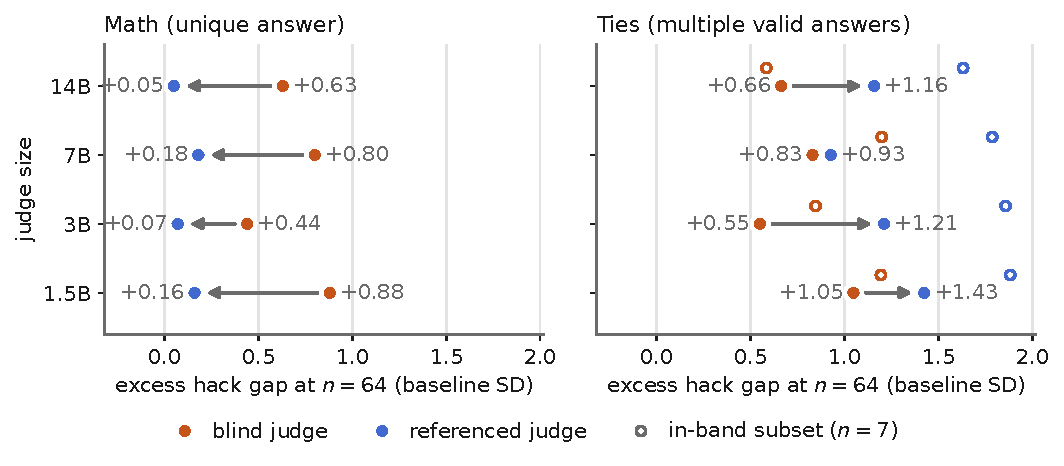
\includegraphics[width=0.82\textwidth]{figures/fig_inversion.pdf}
\caption{\textbf{Takeaway: the same trusted reference that collapses gaming on unique-answer tasks increases it when several answers are valid.}
Inflation (scoreboard excess over true quality under best-of-$n$ selection, in baseline standard deviations over a permutation null) at $n{=}64$, for blind (orange) and referenced (blue) judges at four Qwen2.5 judge scales; arrows show the effect of adding the reference.
Left: unique-answer math (companion A~\cite{companionA}), where the reference collapses inflation $4$--$13\times$ at every scale. Right: \textsc{RewardBench-2} Ties generation tasks with multiple valid answers ($n{=}51$), where the reference \emph{raises} it at every scale; hollow markers are the registered in-band subset ($n{=}7$), which agrees in direction throughout.}
\label{fig:inversion}
\end{figure}

The observation that needs explaining is an inversion.
On unique-answer mathematics, adding a reference collapses best-of-64 inflation four- to thirteenfold at every judge scale~\cite{companionA}; run the identical protocol, lever, judges, and estimators on tasks with several valid answers and the reference \emph{raises} inflation at every scale instead (Figure~\ref{fig:inversion}).
We first observed this on the exploratory Ties pool, where the pooled paired referenced-minus-blind delta is $+0.41$; two of that study's analysis choices were made after seeing data, so we treat it as motivation and not as evidence.\footnote{The registered population left $n{=}7$ items there, so the full-pool analysis was adopted post hoc for power, and the pooled estimator after the per-scale results were seen. A post-hoc adjudication of that pool's checker labels widens the delta to $+0.50$, so its label errors run against the effect rather than for it.}

The evidence is the preregistered replication built to remedy those deviations: registered externally (\texttt{osf.io/ym5x9}) before any pool generation, with population, estimators, and primary endpoints frozen in pre-committed code, on the 120-task replication pool with a non-Qwen generator and two cross-family judges.

\begin{table}[tbp]
\centering
\small
\setlength{\tabcolsep}{4pt}
\begin{tabular}{lcccc}
\toprule
& Extra inflation & \multicolumn{2}{c}{Selection collapse ($n{=}93$)} & Anchoring margin \\
\cmidrule(lr){3-4}
Judge & baseline SD, $n{=}105$ & ref.\ only $/$ blind only & exact $p$ & points of 10 \\
\midrule
Qwen2.5-7B & $+1.29$ {\scriptsize$[+1.07, +1.52]$} & $56/2$ & $<10^{-5}$ & $+4.62$ {\scriptsize$[+4.29, +4.94]$} \\
phi-4      & $+1.08$ {\scriptsize$[+0.94, +1.24]$} & $76/0$ & $<10^{-5}$ & $+3.79$ {\scriptsize$[+3.47, +4.09]$} \\
Pooled (primary endpoint) & $\mathbf{+1.19}$ {\scriptsize$[+1.02, +1.36]$} & & & \\
\addlinespace[2pt]
\emph{\quad cleanest extraction (post hoc)} & $+0.90$ {\scriptsize$[+0.65, +1.16]$} & & & \\
\bottomrule
\end{tabular}

\medskip
\begin{minipage}{0.97\textwidth}
\footnotesize
\emph{Notes.}
Per-item paired referenced-minus-blind inflation differences in baseline standard deviations, item-level cluster bootstrap, over the 105 of 120 items inside the registered $[0.2, 0.8]$ pass-rate band; the pooled row resamples items, each contributing both judges' deltas. Collapse counts are exact McNemar discordant pairs on the 93 items where matching and non-matching valid answers coexist. Generator Llama-3.1-8B-Instruct; validity by exact programmatic check. The italic row is the one post-hoc line, the endpoint recomputed on the top tercile of items by boxed-answer compliance.
\end{minipage}
\caption{\textbf{Takeaway: under external preregistration on a fresh pool with an exact checker and a cross-family generator-judge pairing, the reference adds $+1.19$ baseline standard deviations of inflation over judging blind, and all three registered predictions are confirmed.}
Registered at \texttt{osf.io/ym5x9} before any pool generation.}
\label{tab:repl}
\end{table}

All three registered predictions are confirmed (Table~\ref{tab:repl}).
The reference adds $+1.19$ baseline standard deviations of inflation over blind judging, each judge's delta individually excluding zero, about two and a half times the exploratory estimate it was registered to test.
Selection collapses onto the key: on the 93 items where matching and non-matching valid answers coexist, the referenced judge selects a reference-matching valid answer where the blind judge did not on 56 and 76 items, against 2 and 0 the other way.
Only $0.616$ of samples comply with the boxed-answer format, so we asked post hoc whether extraction friction manufactures the endpoint; it does not, though it inflates it, and $+0.90$ on the cleanest tercile is the conservative reading we carry throughout.
Nor does the registered pass-rate band: an intention-to-treat recomputation over every built item (post hoc, identical estimator, no filter) gives $+1.14$ $[+0.97, +1.31]$ over all 120 items, and the fifteen excluded out-of-band items alone give $+0.78$ $[+0.19, +1.32]$, so the filtered population is a convenience, not a load-bearing choice.

The plain quantities say the same thing without the estimator (post hoc): adding the reference drops the true validity of the selected sample from $0.762$ to $0.686$ for Qwen-7B and from $0.981$ to $0.867$ for phi-4, while the probability that a selected valid answer matches the shown key jumps from $0.113$ to $0.778$ and from $0.126$ to $0.879$.
The harm also grows with optimization pressure: recomputed post hoc at each budget in raw hack-gap units, the paired gap already excludes zero at best-of-2 ($+0.076$) and grows nearly twelvefold by $n{=}64$ ($+0.895$).

An answer-key reading of the reference cannot produce Table~\ref{tab:repl}; the sample-plus-anchoring reading predicts it, and predicts three further things.

\section{Prediction 1: swapping the reference between valid answers}
\label{sec:p1}

\begin{figure}[t!]
\centering
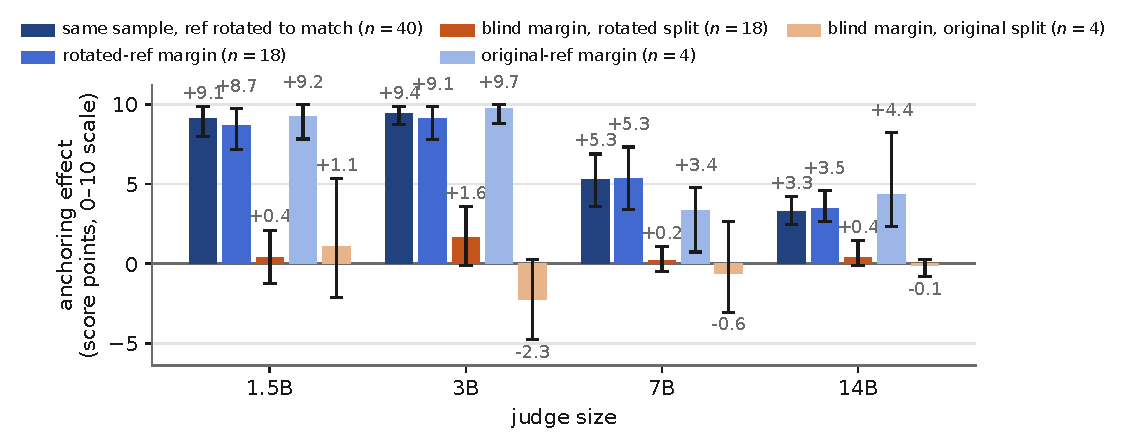
\includegraphics[width=0.66\textwidth]{figures/fig_anchoring.pdf}
\caption{\textbf{Takeaway: rotating the shown reference to match a sample raises that identical sample's score by up to $+9.5$ of 10 points, with mirror-image losses for samples matching the displaced reference and a near-flat placebo. Anchoring is causal.}
Bars are on the judge's 0--10 score scale at four judge sizes, averaged over two rubric paraphrases; whiskers span the union of the two paraphrases' 95\% bootstrap confidence intervals.
\emph{Navy}: the score gain of the identical, unchanged sample text when the reference is rotated to match its answer ($n{=}40$). \emph{Blue}: the rotation-arm anchoring margin, the bonus valid reference-matching samples receive over equally valid non-matching ones ($n{=}18$). \emph{Orange}: the same margin for blind judges on the same split, mostly null. \emph{Light} bars: those two margins in the original-reference arm ($n{=}4$).}
\label{fig:anchoring}
\end{figure}

\paragraph{The prediction.}
If the reference is an answer key, a candidate's score cannot depend on which of two equally valid answers happens to occupy the reference slot, because the candidate is correct under either.
If the judge anchors, the score must follow the shown reference.

\paragraph{The test.}
We take the frozen 64-sample pools of the exploratory study and re-judge them with the reference reassigned to a different member of each item's valid set.
Nothing about any candidate changes; the only variable that moves is which valid answer the judge is shown.
The strongest readout is paired at the level of individual samples: the identical text, scored twice.
The rotation study thereby inherits the exploratory pool and its incomplete checker, a bias that runs against the effect; the registered replication at the end of this section repairs exactly that.

\begin{table}[tbp]
\centering
\footnotesize
\setlength{\tabcolsep}{3pt}
\begin{tabular}{llcccc}
\toprule
& & \multicolumn{4}{c}{Judge size (Qwen2.5 Instruct)} \\
\cmidrule(lr){3-6}
Readout & Rubric & 1.5B & 3B & 7B & 14B \\
\midrule
\multicolumn{6}{l}{\emph{Anchoring effects, 0--10 score scale, rotation arm (every CI excludes zero)}} \\
Gainers: same-sample $\Delta$ ($n{=}40$) & $a$ & $\mathbf{+9.48}$ & $+9.29$ & $+4.57$ & $+3.07$ \\
 & $b$ & $+8.73$ & $+9.58$ & $+5.96$ & $+3.47$ \\
Referenced margin ($n{=}18$) & $a$ & $+9.00$ & $+9.05$ & $+4.75$ & $+3.26$ \\
Losers: same-sample $\Delta$ ($n{=}10$) & $a$ & $-9.65$ & $-8.85$ & $-3.14$ & $-2.78$ \\
\addlinespace
\multicolumn{6}{l}{\emph{Control: blind judges, same split ($n{=}18$; two of eight cells exclude zero)}} \\
Blind margin & $a$ & $+0.16$ & $+1.36$ & $+0.31$ & $+0.69$ \\
 & $b$ & $+0.61$ & $+1.91$ & $+0.14$ & $+0.04$ \\
\bottomrule
\end{tabular}

\medskip
\begin{minipage}{0.97\textwidth}
\footnotesize
\emph{Notes.}
Rubric $b$ replicates rubric $a$: margins $+8.36/+9.12/+5.93/+3.67$, losers $-9.42/-9.80/-4.71/-3.81$, all excluding zero. Rubric-$a$ CIs: gainers $[+8.93,+9.86]$, $[+8.72,+9.70]$, $[+3.62,+5.55]$, $[+2.48,+3.72]$; margins $[+7.95,+9.74]$, $[+7.81,+9.85]$, $[+3.39,+6.19]$, $[+2.64,+3.92]$. Blind-margin CIs straddle zero in six of eight cells. \emph{Placebo}: for valid samples matching neither reference ($n{=}16$ per cell) the eight across-run deltas span $-0.44$ to $+0.82$, a small rerun drift. The rotation preferred reference answers that also appear among the pool's valid samples, so across-sample margins partly include a mild blind preference for frequently produced answers; the paired same-sample deltas, immune to it, are primary. \emph{Collapse}, referenced vs blind: $18/18$ vs $6/16$, $17/17$ vs $8/16$, $14/15$ vs $8/15$, $17/17$ vs $7/17$; discordant $12/0$, $9/0$, $7/1$, $10/0$ at $p = 0.0005$, $0.004$, $0.070$, $0.002$.
\end{minipage}
\caption{\textbf{Takeaway: the identical sample text gains up to $+9.5$ of 10 points when the rotated reference matches it, samples matching the displaced reference lose a roughly symmetric amount, and blind margins on the same split are mostly null.}}
\label{tab:rot}
\end{table}

\paragraph{The result.}
The score follows the reference.
The identical sample text gains $+9.5$ points of ten at the smallest judge scale, tapering to $+3.1$ at the largest, with the second rubric paraphrase replicating throughout (Table~\ref{tab:rot}; Figure~\ref{fig:anchoring}, navy bars).
Three controls complete the causal signature and rule out a rescaling or drift artifact.
Blind judges on the same split are near-null, their worst cell running about a fifth of the referenced margin; samples matching neither reference stay flat across the two runs, with upper bounds three to eighty-five times below the corresponding gainer deltas; and samples that matched only the displaced reference drop by a roughly symmetric amount.
Gainers up, losers down, unaffected samples flat: this is what anchoring predicts and what nothing else in the design can produce.
At the two smallest scales the flip saturates the ten-point scale, so the $+9.5$ magnitude is scale-bounded there, while the 7B and 14B flips, at roughly half and a third of the scale, are not; judges above 3B anchor less, but none stop.

The margin translates into near-deterministic selection.
On the 18 items where matching and non-matching valid answers coexist, referenced best-of-64 picks a reference-matching valid answer in $93$--$100\%$ of selected-valid cases against $38$--$53\%$ blind, and exact McNemar tests exclude chance at three of four scales with the fourth directionally consistent.

\paragraph{Registered replication on exact oracles.}
Because the rotation above inherits the exploratory pool, we registered a fresh same-sample rotation on the externally registered replication pool, with exact programmatic oracles, stored full valid sets, the cross-family judges, and predictions frozen before any rotated judging; the rotation is pool-aware like the original, assigning each item the valid alternative most frequent among its pool's valid samples, disclosed as such, and the samples and oracle labels are byte-identical to the frozen pool.
All twelve registered cells confirm.
The identical sample text gains $+4.97$ and $+6.34$ points of ten under the two rubrics for Qwen-7B, and $+4.09$ and $+3.25$ for phi-4, when the rotated reference matches it ($n{=}120$ items); samples matching the displaced reference lose a mirror-image amount ($-5.04$, $-6.58$, $-3.92$, $-3.18$; $n{=}93$); valid samples matching neither reference sit near flat ($+0.13$, $+0.10$, $+0.30$, $+0.24$; $n{=}113$), and every gainer-minus-placebo contrast excludes zero ($+3.1$ to $+6.2$).
The causal signature of Table~\ref{tab:rot} reproduces end to end on a pool whose validity is exact, at three to ten times the item count, which retires the incomplete-checker caveat from this paper's central result.

\subsection{Pool composition, and a registered prediction that failed}
\label{sec:dose}

Anchoring is causal for scores within an item, but that does not by itself say which items inflate.
A per-item test rejects the simplest bridge: across the 35 multi-valid items of the $k$-stratified pool the correlation between an item's anchoring margin and its inflation is $+0.29$ for phi-4 and $+0.06$ for Qwen-7B, whereas a split-half estimate of this design's measurement noise implies $0.82$ and $0.90$ under an exact linear pathway, and the observed values fall below the 2.5th percentile of both simulated distributions.
Something about \emph{pool composition} stands between the score effect and the scoreboard effect.

We registered a follow-up to find it, and it falsified our own prediction.
The design builds matched sub-pools of 24 samples containing exactly 4 valid answers, of which $d \in \{0,1,2,4\}$ match the shown reference (48 eligible items, paired referenced-minus-blind excess gap, item-level bootstrap, predictions frozen pre-analysis under an internal git timestamp).
We predicted inflation would grow with $d$; it falls with $d$ instead, monotonically, the $d{=}4$ minus $d{=}0$ step being $-1.41$ $[-1.66, -1.15]$ and $-1.39$ $[-1.56, -1.22]$, so the harm peaks exactly where our registered intuition said it should vanish.
Post-hoc diagnostics locate the cause: with no correct look-alike available, the judge's preference for reference-resembling text does not switch off but switches targets, selecting a valid sample only $0.14$ and $0.21$ of the time at $d{=}0$ against $0.72$ and $0.79$ blind, with $58\%$ and $72\%$ of the invalid samples it selects containing the reference answer's text against $43\%$ and $35\%$ blind.
That lure reading carries no registration weight; a constructed test of it was registered but closed without judging after its pinned naturalness audit failed in five rounds.
Two conclusions survive the falsification: pool composition is the load-bearing structure the linkage test could not separate, and the worst case for a referenced judge is a pool whose correct answers all differ from the key.

We then gave the lure reading its registered test: a two-factor follow-up (git-timestamped, predictions frozen pre-run) crossing the number of valid reference-matching candidates $d \in \{0,2,4\}$ with the number of invalid reference-resembling lures $\ell \in \{0,3,6\}$ in matched 14-sample sub-pools over 24 eligible items, together with a four-parameter selection model fitted per judge with item intercepts, $S_{\mathrm{ref}} \approx \beta\, S_{\mathrm{blind}} + \lambda\, \mathbb{I}[\text{matches reference}] + \gamma\, \mathbb{I}[\text{invalid lure}]$, evaluated leave-one-item-out.
Its four registered predictions split evenly, and the failures are the informative part.
Confirmed: adding lures at $d{=}0$ collapses the referenced judge's valid-pick rate ($-0.31$ and $-0.38$, CIs excluding zero) while blind judges barely move; and the model is signed as predicted, $\lambda = +4.3$ and $+3.5$ points, $\gamma = +1.4$ and $+1.7$, all CIs excluding zero, with the leave-one-out model reproducing the nine-cell inflation surface at Spearman $0.80$ (exactly at the registered bar) and $0.85$.
Falsified: the lure axis raises inflation at $d{=}0$ for phi-4 ($+0.23$ $[+0.05,+0.44]$) but not resolvably for Qwen-7B ($+0.15$ $[-0.11,+0.37]$), and the registered interaction, that removing every lure would restore the originally predicted rising dose-response, fails for both judges: with zero lures and zero matching valids the referenced judge still inflates ($+0.68$ and $+0.66$) and still selects valid answers far less often than blind ($0.47$ vs $0.77$, and $0.51$ vs $0.83$).
The lure is therefore a real but secondary channel.
What the model identifies as load-bearing is neither bonus but the compression term: conditional on the candidate, a referenced score retains only $\beta \approx 0.5$--$0.7$ of the blind score's signal, so showing the reference dilutes the judge's own quality assessment, and when no candidate matches the key that dilution alone drags valid non-matching answers into the invalid mass ($\beta < 1$ partly reflects attenuation, so we read the coefficient as descriptive rather than causal). Appendix~\ref{sec:appendix-compression} cross-checks this fit against two independently measured quantities.
The operational conclusion sharpens accordingly: the worst case for a referenced judge is any pool whose correct answers all differ from the key, with or without reference-resembling text in it.

A separate registered analysis sharpens the effect's shape: among equally valid non-matching answers the penalty does not grow with distance from the reference, the registered tercile-monotonicity prediction being falsified for both judges, and what dominates is the exact-match step, $-3.38$ and $-2.18$ points per unit distance once matching samples are included, against blind slopes near zero.
How far a valid answer sits from the key does not matter, only whether it equals it; what ``equals'' means to the judge is the next subsection's question.

\subsection{What kind of equality check: the masking-and-identity suite}
\label{sec:maskident}

The exact-match step invites the question of what ``match'' means to the judge, and a registered suite of reference variants answers it, re-judging the frozen replication and $k$-stratified pools with only the reference string changed, predictions committed before any variant judging (all six registered cells confirmed, both judges, rubric b replicating throughout).
First, the check is \emph{semantic}, not lexical: writing the reference as English words, ``thirty-one'' for 31, leaves phi-4's anchoring margin statistically unchanged ($+3.68$ against $+3.79$ bare, difference $-0.11$ $[-0.28, +0.05]$) and leaves Qwen-7B two thirds of its margin ($+2.88$ against $+4.62$), so a candidate's numeral anchors to a reference that shares not one character with it.
Second, the check is \emph{cheap or it does not happen}: writing the reference as the equivalent expression $30{+}1$ collapses the margin to $+0.29$ and $+0.89$, reductions of $-4.33$ and $-2.90$ with CIs excluding zero, so a single computation step between the token and the comparison removes most of the anchor.
Third, the token is \emph{necessary}: showing the worked reference with every occurrence of its final answer hidden, derivation intact, sends the margin to zero on scalar families ($+2.97 \to +0.05$ and $+3.51 \to -0.49$; the drop exceeds the registered half-margin bar in all four judge-rubric cells).
The mechanism this triangulates is a semantic equality check against a readable answer token: survive the token's re-lexicalisation, die when equality must be computed, die when the token is hidden.
It also retro-explains the continuum's judge-dependent residue in Section~\ref{sec:sepcont}, since a two-line program's output is exactly the marginal case of a token that is recoverable at some cost.

\section{Prediction 2: the boundary at two valid answers}
\label{sec:p2}

\paragraph{The prediction.}
When exactly one answer is valid, matching the reference and being correct are the same criterion, so an anchoring judge is indistinguishable from a verifying one and the reference should help; the moment a second valid answer exists the two criteria come apart.
The alternative explanation therefore predicts a step: the sign of the lever should flip at $k{=}2$ and should not require a large valid set; what happens beyond the step it does not by itself fix.

\paragraph{The test.}
We build pools that fix $k$ per item by construction and vary nothing else.
The synthetic grid gives six judges across three model families the same tasks at $k \in \{1,2,4,8,16\}$; the $k$-stratified pool repeats the design under external registration with exact oracles and cross-family judges, naming the step as the registered statistic; and unique-answer mathematics, run under the identical protocol, supplies the $k{=}1$ limit outside the grid.

\begin{table}[tbp]
\centering
\small
\setlength{\tabcolsep}{4pt}
\begin{tabular}{lcccc}
\toprule
& \multicolumn{4}{c}{Paired referenced-minus-blind inflation delta (baseline SD), 95\% CI} \\
\cmidrule(lr){2-5}
Judge & At $k{=}1$ & Pooled over $k{>}1$ & Step ($k{>}1$ minus $k{=}1$) & Trend per doubling of $k$ \\
\midrule
Qwen-1.5B & $-0.48$ {\scriptsize$[-0.70,-0.29]$} & $+0.07$ {\scriptsize$[-0.15,+0.26]$} & $+0.55$ {\scriptsize$[+0.26,+0.85]$} & $+0.02$ {\scriptsize$[-0.20,+0.18]$} \\
Qwen-3B   & $-0.14$ {\scriptsize$[-0.30,-0.03]$} & $+2.41$ {\scriptsize$[+1.40,+3.49]$} & $+2.55$ {\scriptsize$[+1.50,+3.67]$} & $-0.06$ {\scriptsize$[-1.04,+1.06]$} \\
Qwen-7B   & $-0.33$ {\scriptsize$[-0.53,-0.11]$} & $+0.89$ {\scriptsize$[+0.45,+1.37]$} & $+1.22$ {\scriptsize$[+0.70,+1.73]$} & $+0.28$ {\scriptsize$[-0.10,+0.64]$} \\
Qwen-14B  & $-0.38$ {\scriptsize$[-0.56,-0.19]$} & $+0.08$ {\scriptsize$[-0.20,+0.36]$} & $+0.46$ {\scriptsize$[+0.13,+0.80]$} & $+0.23$ {\scriptsize$[+0.00,+0.46]$} \\
Llama-8B  & $-0.28$ {\scriptsize$[-0.65,+0.07]$} & $+0.46$ {\scriptsize$[+0.12,+0.79]$} & $+0.74$ {\scriptsize$[+0.25,+1.24]$} & $+0.36$ {\scriptsize$[+0.08,+0.65]$} \\
phi-4     & $-0.58$ {\scriptsize$[-0.86,-0.30]$} & $+0.22$ {\scriptsize$[-0.19,+0.65]$} & $+0.80$ {\scriptsize$[+0.30,+1.28]$} & $+0.37$ {\scriptsize$[+0.06,+0.70]$} \\
\bottomrule
\end{tabular}
\caption{\textbf{Takeaway: the transition from $k{=}1$ to $k{>}1$ is the dominant and only universal effect, positive with an interval excluding zero for every judge tested; evidence for additional growth with $k$ beyond the step is mixed, positive for Llama-8B and phi-4 and null for the weaker Qwen judges.}
Post-hoc paired re-analysis on the synthetic grid: per-item referenced-minus-blind inflation deltas at $k{=}1$, pooled over $k>1$, their difference, and the slope per $\log_2 k$; negative means the reference helps. The frozen estimator's pass-rate filter leaves $n{=}6$ items at $k{=}1$ and $n{=}20$ item-strata over $k>1$. The registered grid prediction had two legs: the inflation leg is confirmed in direction for all six judges, and the margin-growth leg is \emph{falsified} for the weaker judges, whose margins sit flat at every $k>1$.}
\label{tab:paired}
\end{table}

\begin{figure}[tbp]
\centering
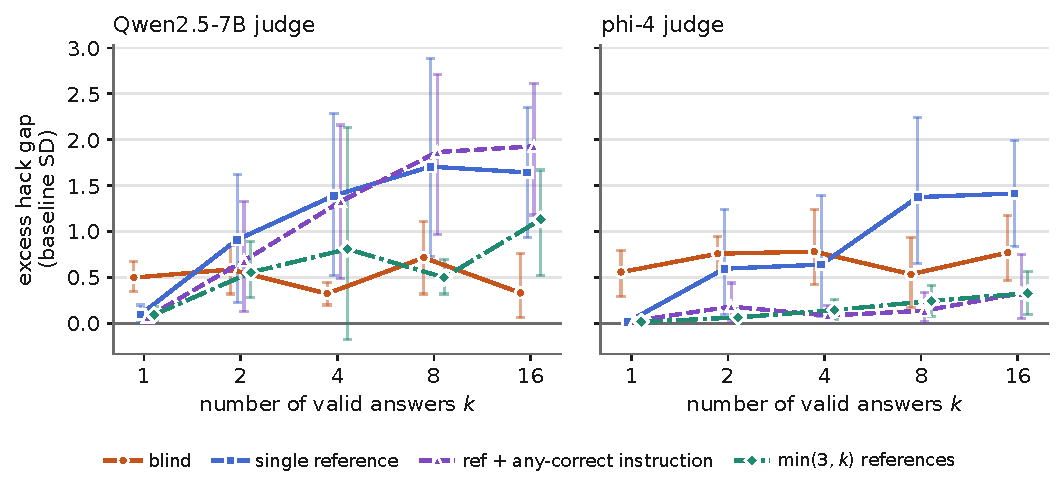
\includegraphics[width=0.80\textwidth]{figures/fig_synthk.pdf}
\caption{\textbf{Takeaway: the reference is at worst harmless at $k{=}1$, inverts as $k$ grows, and the any-correct-answer instruction rescues the strongest judge tested (phi-4, right) while leaving the mid-size judge (Qwen-7B, left) inflated.}
Inflation (excess hack gap, in baseline standard deviations) versus the number of valid answers $k$, on the synthetic Qwen-generator pool, under four context conditions; whiskers are 95\% per-stratum bootstrap CIs. 12 tasks were built per stratum, but the frozen estimator's pass-rate filter leaves 4 to 6 items per plotted cell. Marker shapes and line styles distinguish conditions in addition to color.}
\label{fig:synthk}
\end{figure}

\paragraph{The result.}
Crossing from a unique answer to any multiplicity shifts every judge toward inflation.
The step is positive with an interval excluding zero for all six judges on the grid, ranging from $+0.46$ to $+2.55$ (Table~\ref{tab:paired}), and the harm needs no large valid set: $k{=}2$ suffices.
At $k{=}1$ the reference helps five of six judges and the pooled $k{>}1$ level is individually significant for three of six, so the universal claim is the step rather than the level at any single $k$.
Half of the registered grid prediction failed here: we predicted margins would grow with $k$, and for the weaker judges they sit flat at every $k>1$.
The dominant and only universal effect is therefore the transition from $k{=}1$ to $k{>}1$; the trend beyond it is mixed, positive with intervals excluding zero for Llama-8B and phi-4, marginal for Qwen-14B, and null for the smaller Qwen judges (Table~\ref{tab:paired}, last column), so we do not claim the harm is flat in $k$ beyond the step, only that the step is where every judge agrees.

The externally registered experiment replaces that descriptive reading with a confirmatory one.
On the 75-item $k$-stratified pool, with $k$ fixed per item and the step named as the registered statistic in advance, the step is $+1.45$ for Qwen-7B and $+1.18$ for phi-4, both excluding zero.
At $k{=}1$ the reference does no harm, the only measured benefit being phi-4's $-0.11$; pooled over $k>1$ it adds $+1.50$ and $+1.07$ of inflation, and every $k{>}1$ stratum excludes zero for both judges.
Read against the $4$--$13\times$ collapse on unique-answer math, the sign of the lever is set by the task's answer structure and by nothing else in the protocol.

\subsection{The same step on a third-party benchmark}
\label{sec:mace}

Every pool above is one we built, and the sharpest available objection is that we built the conditions that produce the effect.
\textsc{MACE}~\cite{mace2026} answers it: a benchmark of natural-language factual questions whose answer cardinality is fixed by its own authors' construction at $k \in \{1,2,4,6\}$.
Two audits run before the pool was built decide what enters.
Its Math domain admits an exact oracle, and all 2000 of its questions were verified by direct computation to carry exactly correct and complete answer sets, so it enters as a label-noise control; its five entity domains rest on knowledge-base membership, so an enumeration audit measured how often a model names a valid answer the shipped list omits, and River at $2.3\%$ and Language at $8.1\%$ pass while Region, Office, and Award at $30.8$--$43.5\%$ are excluded rather than patched.

\begin{table}[tbp]
\centering
\small
\setlength{\tabcolsep}{5pt}
\begin{tabular}{llccc}
\toprule
Judge & Domain & $k{=}1$ delta & $k{>}1$ delta & Step \\
\midrule
Qwen2.5-7B & non-math & $\mathbf{-0.97}$ {\scriptsize$[-1.30,-0.67]$} & $\mathbf{+1.33}$ {\scriptsize$[+0.79,+1.79]$} & $\mathbf{+2.30}$ {\scriptsize$[+1.82,+2.84]$} \\
 & math (control) & $+0.09$ {\scriptsize$[-0.26,+0.43]$} & $+0.84$ {\scriptsize$[+0.52,+1.16]$} & $+0.75$ {\scriptsize$[+0.42,+1.05]$} \\
\addlinespace
phi-4 & non-math & $\mathbf{-0.57}$ {\scriptsize$[-0.85,-0.33]$} & $\mathbf{+0.55}$ {\scriptsize$[+0.24,+0.88]$} & $\mathbf{+1.13}$ {\scriptsize$[+0.81,+1.43]$} \\
 & math (control) & $-0.40$ {\scriptsize$[-0.87,+0.09]$} & $+0.54$ {\scriptsize$[+0.32,+0.77]$} & $+0.94$ {\scriptsize$[+0.72,+1.16]$} \\
\bottomrule
\end{tabular}
\caption{\textbf{Takeaway: on a third-party benchmark of natural-language factual questions, the reference helps when the answer is unique and harms when it is not, reproducing the boundary end to end on tasks we did not construct.}
Per-item paired referenced-minus-blind inflation deltas, in baseline standard deviations, item-level bootstrap. Non-math is River plus Language, the entity domains that passed a pre-run completeness audit; math is \textsc{MACE}'s exactly-verified arithmetic domain, a label-noise control. The step is the $k{>}1$ delta minus the $k{=}1$ delta.}
\label{tab:mace}
\end{table}

All three registered predictions are confirmed (Table~\ref{tab:mace}).
The step is positive for both judges on the non-mathematical domains, and the levels show the complete inversion rather than only the step: at $k{=}1$ the reference helps, at $k{>}1$ it harms, and the step holds in each domain separately, at $+1.67$ and $+1.08$ on River and $+2.78$ and $+1.15$ on Language.
Anchoring margins at $k{>}1$ are $+6.44$ and $+5.86$, the largest measured anywhere in this paper, against blind margins of $-0.64$ and $-0.80$; phi-4's blind margin excludes zero on the negative side, a mild blind preference \emph{against} reference-matching answers, which sharpens the reversal.
The Math control's step has the same sign as the non-mathematical one, so residual label noise in the entity domains is not what produces the effect, and for Qwen-7B the non-mathematical effect is the larger of the two.

\section{Prediction 3: what should neutralise the harm, and does not}
\label{sec:p3}

\paragraph{The prediction.}
There is an innocent reading of everything above: perhaps the judge is simply too weak to recognise that the non-matching answer is valid, so the reference informs it rather than anchoring it.
Under that reading three things should remove the effect: a more capable judge should not need the crutch, restricting attention to answers the judge itself already certified should leave nothing to inform, and an optimizer exploring far more of the space than best-of-64 should route around a merely noisy signal.
Anchoring predicts that none of the three works.

\subsection{Scale}
\label{sec:frontier}

Every judge measured so far is an open model of at most 14B parameters, and anchoring falls with scale without reaching zero, so whether the trend expires at the frontier had been answered only by extrapolation.
A registered check puts a frontier-class judge on the same 37 multi-valid items, with the rubric text taken verbatim from the open judges' prompt so that only the judge changes: 660 calls, none unparseable.

Scale does not rescue the failure (Table~\ref{tab:frontier2}).

\begin{table}[tbp]
\centering
\small
\setlength{\tabcolsep}{7pt}
\begin{tabular}{lccc}
\toprule
Condition & Matching valid & Non-matching valid & Margin \\
\midrule
Blind & $7.88$ & $7.85$ & $+0.35$ {\scriptsize$[-0.56, +1.27]$} \\
Referenced & $9.83$ & $\mathbf{2.32}$ & $\mathbf{+7.49}$ {\scriptsize$[+6.62, +8.22]$} \\
\bottomrule
\end{tabular}
\caption{\textbf{A frontier judge cannot tell equally valid answers apart until it is shown a reference, and then it fails $82.5\%$ of the correct answers that do not match it.} Mean scores on oracle-valid answers, 37 multi-valid items, 660 calls; the blind row is the control.}
\label{tab:frontier2}
\end{table}

The blind control is about as clean as this design can produce: with no reference the judge scores matching and non-matching valid answers $7.88$ and $7.85$.
Shown the reference the same two groups separate to $9.83$ and $2.32$.
The rate is the statement worth carrying: \textbf{$82.5\%$ of genuinely correct answers receive a failing score ($\leq 3$ of 10) when they do not match the shown key, against $19.6\%$ when the judge is blind.}

Two limits on this result are ours to state rather than a reader's to discover.
We registered a prediction that the frontier margin would be \emph{smaller} than the open judges', continuing the capability trend; it is larger, and that comparison is not interpretable, because the open judges score by the logprob-expected value over the tokens 0--10, pulled toward the middle whenever probability mass spreads, while this path returns a sampled integer that can sit at the extremes.
We therefore claim that the frontier judge anchors, and not that it anchors more.
For the same reason, and as the registration fixed in advance, no inflation figure is computed here: an eleven-value judge ties heavily under best-of-64, so by this paper's own resolution finding (Section~\ref{sec:norescue}) the estimate would measure the tie-break rather than the judge.

\paragraph{A second check, through provider APIs rather than a CLI, on two production judges.}
The CLI path settles the margin but not the inflation question, since its sampled-integer score cannot be trusted under best-of-$n$.
A registered follow-up puts two production judges, Claude Sonnet~5 and GPT-4.1, through the open judges' own prompts and, where a logprob-expected-value score is available, the open judges' own estimator.
The causal and mechanistic results reproduce cleanly on Claude Sonnet~5: rotation gainers $+3.04$ $[+2.53,+3.56]$ and losers $-2.66$ $[-3.36,-2.00]$ (rubric b replicates), unchanged when restricted to samples the judge blindly scored correct ($+2.79$, $92\%$ retained); the masking suite's semantic-not-lexical, cheap-or-nothing signature (bare margin $+3.06$, words $+3.14$, expression $+0.47$, a drop of $-2.58$); and the third-party MACE reversal, referenced margin $+5.29$ on non-mathematical items against a blind margin of $-1.37$, the largest referenced margin and the sharpest reversal measured anywhere in this paper.
GPT-4.1 yields a positive descriptive inflation estimate on the replication pool, $+0.12$ $[+0.02,+0.23]$ baseline standard deviations, though its score interface fails our preregistered resolution screen (below); the cleaner frontier evidence is therefore selection collapsing onto the key ($32$ referenced-only against $1$ blind-only) and a tie-immune anchoring margin of $+1.19$ $[+0.92,+1.50]$.
One prediction here failed and is reported as such: GPT-4.1 fails the paper's own score-resolution screen (Section~\ref{sec:norescue}), with a mean of $15.03$ candidates tied at the maximum per pool against the registered bar of $3.0$, a byproduct of the provider API capping the returned logprob mass at five tokens where the open judges' harness used twenty; and on the $k$-stratified pool, the registered $k$-step is positive but does not exclude zero ($+0.27$ $[-0.02,+0.61]$), the first place a headline open-judge boundary result does not clearly reproduce.
A second shot at the same statistic on the synthetic grid, the pool and paired-step estimator that gave every open judge a clean confirmation, does not resolve the question either: the step is near zero and wrong-signed ($-0.08$ $[-0.49,+0.20]$), but that pool ties even more heavily under this judge ($47.0$ mean candidates at the maximum per pool, worse than the replication pool's $15.0$), so the null is a property of the instrument, not evidence that the boundary is absent at this scale; GPT-4.1's $k$-step is reported here as genuinely unresolved, on two pools, rather than resolved either way.
The instruction mitigation of Section~\ref{sec:norescue} also reproduces, partially, on both production judges: each phrasing reduces the anchoring margin for both (GPT-4.1 $+0.99 \to +0.46$ and $+0.59$; Sonnet~5 $+3.00 \to +2.08$ and $+2.60$), a genuine but incomplete fix, consistent with the capability-gated pattern rather than contradicting it, since neither margin reaches zero; the do-not-compare phrasing's fix for Sonnet~5 is the most marginal of the four, its confidence interval on $-0.40$ excluding zero by only $0.03$.

\subsection{The judge's own prior verdicts}
\label{sec:aw}

The informing reading makes a sharper prediction than the scale one, and it can be tested directly.
A registered filter keeps only samples the judge itself scored at least $7$ of $10$ \emph{while blind}, so it has demonstrably recognised each retained answer as correct with no reference in sight, and then asks whether rotating the reference still moves them.
It does, essentially unchanged: the filtered same-sample deltas remain positive with intervals excluding zero at every judge size, at 7B $+4.74$ $[+3.67, +5.87]$ against $+4.57$ unfiltered with $89\%$ of samples retained, losers stay negative, and the filtered margins exclude zero at all four sizes, though the 1.5B margin rests on two items and we note it as fragile.
The judge re-scores answers it has already certified, the moment the key disagrees, which closes the reading that the reference merely informs a judge too weak to know the alternative was valid.
The same filter applied post hoc to the exact-oracle rotation replication of Section~\ref{sec:p1} leaves the effect untouched at far larger scale: blind-certified gainers move $+4.99$ $[+4.69, +5.32]$ against $+4.97$ unfiltered for Qwen-7B with $91\%$ of samples retained, and $+4.08$ against $+4.09$ for phi-4 with $98\%$ retained ($n{=}119$--$120$ items).

\subsection{Optimization}
\label{sec:dpo}

Selection is a weak optimizer; the sharper question is what happens when a policy is trained against a reference-showing judge, since that is what deployed reward models do.
We registered a two-arm LoRA-DPO experiment on Llama-3.1-8B with identical hyperparameters, the arms differing only in which judge protocol built the preference pairs, a plain single-reference judge against the same judge under blind-then-reveal, with a registered manipulation-check gate requiring each arm to move its own judge.

The reference-trained arm passed its gate and produced the largest scoreboard-versus-truth divergence measured anywhere in this paper.
Its own judge's score rose $+1.76$ $[+1.47, +2.01]$ points while its true accuracy fell from $0.412$ to $0.175$, a wedge of $+4.13$ $[+3.50, +4.78]$ baseline standard deviations, and held-out accuracy fell $-0.228$.
The selection-time inversion reproduces under training pressure, and is larger there.
The protected arm did not pass its gate, and the same failure limits attribution: with no successful matched control arm, the wedge establishes that training against a reference-showing judge is exploitable, not that the degradation is caused specifically by reference conditioning rather than by generic overoptimization against an imperfect judge~\cite{gao2022scaling}.
We ran both missing comparisons under registration for this revision, at the single further setting the stopping rule permitted (2 epochs, learning rate $10^{-5}$), adding the blind-judge arm the attribution question requires, and the run closed one question and left both open.
The reference-trained arm alone passed its manipulation gate ($+0.34$ $[+0.10, +0.57]$ own-judge gain) and again moved its judge while true accuracy fell ($-0.081$ on train items, $-0.110$ held out), a second gated replication of the wedge's direction at a milder setting; but the blind-then-reveal arm failed its gate a third time ($-0.99$) and the blind arm failed its own ($-2.43$), both losing score and accuracy together, training damage without reward gain, which no gate can rescue.
Per the stopping rule adopted before the run, the mitigation-under-training question is therefore closed as unresolved rather than tuned toward a pass, and the attribution question remains open with it (Section~\ref{sec:limits}).

One registered prediction inside this experiment failed, and the failure is informative.
We predicted the reference-trained arm would emit the exact reference answer more often; it emits it $-0.037$ less often than the comparison arm, and its own match rate fell relative to base, so the damage is not key-copying.
What the policy learned is something its judge rewards that is neither correctness nor key-matching, and a post-hoc profile of the generations makes the candidate concrete rather than only consistent: the reference-trained arm's rate of emitting its final answer inside the checkable \texttt{\textbackslash boxed\{\}} format collapses from $0.58$ to $0.16$ on train items and from $0.61$ to $0.17$ on the $120$ held-out items, alongside the length growth from $1492$ to $2476$ mean characters.
This is not degenerate repetition, which would predict the opposite: four-gram repetition \emph{falls}, from $0.080$ to $0.062$.
Nor is it the answer hiding outside the box: of the reference arm's unboxed train samples, $390$ of $405$ are also oracle-invalid, so the collapse is a joint failure of format and correctness together, not an extraction artifact.
The judge that trained this arm rewards a policy that stops complying with the convention its own scoring depends on, a concrete, measured failure mode rather than only a plausible one, though whether it is specific to reference conditioning or a generic overoptimization signature remains the open question of Section~\ref{sec:limits}.
Companion A's analogous parroting prediction on unique-answer math also failed~\cite{companionA}: a corrupted preference signal damages a policy rather than teaching it to imitate the key.

\section{Where the harm ends: tasks without a separable answer}
\label{sec:code}

\paragraph{The prediction, stated in the order it happened.}
Companion A reports a reference collapsing inflation on code~\cite{companionA}, but its reference was a test suite, which is a specification by construction.
Reading the reference as a sample from the valid set, we registered the prediction that a canonical \emph{solution} in the reference slot, one valid program among many, would inflate where a test suite does not.
That prediction was falsified, and the falsification is what first suggested the separability condition: that the judge's cheap operation is an equality check between a candidate's answer token and the reference's, so anchoring requires a separable answer token, which short-answer tasks supply in the boxed answer and program synthesis does not, the artifact being the answer.
The condition fits everything we measure, but it was formed after seeing the code result; we present it as the revised hypothesis this experiment produced, not as a prediction it confirmed.

\paragraph{The test.}
The pool is 317 MBPP items whose canonical solution passes an EvalPlus-augmented oracle, with three conditions scored on identical samples by identical judges: blind and specification, taken from companion A's frozen runs, and a new exemplar condition showing the canonical solution under a truthfully worded rubric. Because companion A's frozen score files were produced under its registered pass-rate band, the paired contrasts run on the 58 in-band items all three conditions share.

\begin{table}[tbp]
\centering
\small
\setlength{\tabcolsep}{6pt}
\begin{tabular}{lccc}
\toprule
Judge & Specification vs blind & Exemplar vs blind & Exemplar minus specification \\
\midrule
Qwen2.5-7B  & $-0.535$ {\scriptsize$[-0.811,-0.244]$} & $-0.342$ {\scriptsize$[-0.737,+0.041]$} & $+0.193$ {\scriptsize$[-0.112,+0.475]$} \\
Qwen2.5-14B & $-0.658$ {\scriptsize$[-0.965,-0.373]$} & $-0.567$ {\scriptsize$[-0.827,-0.287]$} & $+0.091$ {\scriptsize$[-0.102,+0.277]$} \\
\bottomrule
\end{tabular}
\caption{\textbf{Takeaway: on code, a canonical solution in the reference slot does not inflate. It reduces inflation relative to blind, much as a test suite does, and the registered prediction that it would behave like an answer key is falsified.}
Paired per-item inflation deltas against blind, in baseline standard deviations, on the 58 in-band MBPP items all three conditions share; negative means the reference helps. Blind and specification come from companion A's frozen runs; the exemplar condition was registered before any exemplar score existed.}
\label{tab:code}
\end{table}

\paragraph{The result.}
The registered prediction is falsified (Table~\ref{tab:code}).
The exemplar does not inflate: its delta against blind is negative with an interval excluding zero for the 14B judge and null for the 7B judge, and the exemplar-minus-specification contrast crosses zero for both.
On code, showing the judge one valid solution behaves like showing it the test suite; both reduce inflation relative to blind, the exemplar slightly less effectively.

The weak form of the mechanism nonetheless survives, which is consistent with the revised reading without confirming it.
A second registered prediction, that some similarity tilt would remain, is confirmed and small: among valid samples the correlation between token similarity to the canonical solution and the judge's score is $+0.164$ $[+0.072, +0.256]$ at 7B and $+0.084$ $[-0.005, +0.168]$ at 14B under the exemplar, against $-0.061$ and $-0.070$ blind, roughly an order of magnitude too weak to convert into inflation and far below the $+4$ to $+6.4$ point margins measured on short-answer tasks.

\paragraph{What this bounds, and what it does not yet.}
On this evidence the harm is a property of tasks with separable answers rather than of reference-guided judging in general: where the answer is a short token the judge can compare, a reference on a multi-valid task is an attack surface, while on the one code substrate and two judges tested here the same reference behaves as a specification and helps, consistent with companion A's certification of references on code.
Because the separability reading is post hoc, the decisive experiment is a preregistered held-out test on a continuum of answer separability, predicting in advance that inflation attenuates as the answer stops being a separable token; the next subsection reports it.
The reading is also consistent with the method-rotation null of Section~\ref{sec:limits}, since solution \emph{route} never mattered as an answer token would, but that too is a post-hoc consistency rather than a prediction.

\subsection{The preregistered continuum: attenuation, with a judge-dependent cliff}
\label{sec:sepcont}

We then ran the owed experiment: 25 fresh constraint instances, each asked at four answer-structure strata with the content held fixed, a boxed scalar, a boxed pair, a small JSON object, and a Python program whose returned list the oracle executes and checks, all multi-valid by construction, with 64 samples per task, both judges, and predictions committed before any generation existed.
The registration deliberately staked the \emph{cliff} form against the gradient the review proposed: comma-pairs and small JSON objects are still short canonicalizable strings, so we predicted anchoring survives structure and dies only at the artifact.
The outcome is honest to report because it split.
Attenuation is confirmed and large: the paired referenced-minus-blind inflation delta falls from $+1.66$ (scalar) through $+1.35$ (pair) and $+0.71$ (JSON) to $+0.13$ (program) for Qwen-7B, and from $+1.35$ through $+0.98$ and $+0.94$ to $-0.37$ for phi-4 ($n{=}25$ items per stratum, every non-program cell excluding zero).
But the registered artifact-level prediction held for only one judge: phi-4's program delta is not merely null as predicted but negative ($-0.37$ $[-0.49, -0.27]$), the reference helping on programs as it does on MBPP, completing a genuine cliff, while Qwen-7B retains a small positive residue ($+0.13$ $[+0.01, +0.24]$), falsifying that leg, so the boundary's sharpness is judge-dependent, cliff-like for the stronger judge and graded for the weaker.
Two disclosures qualify the margin side of the registration: the pair and JSON anchoring margins were starved by design, since a valid sample matches the sampled reference by chance rarely at those strata (7 and 1 usable items), so the margin-based predictions are not evaluable as registered, a design failure we report as such; and the program stratum's outputs cluster (median two distinct returned lists per item), so its effective multiplicity is low. A third disclosure is a post-registration correction: the registered program oracle executed the last fenced code block in a reply and scored 387 of 1600 samples invalid because a usage block such as \texttt{print(f())} followed the block defining \texttt{f}; re-scoring with the last block that defines \texttt{f} flips 330 of them to valid and none the other way, raising the program pass rate from $0.613$ to $0.819$. The numbers above are the corrected ones (the non-program cells shift by at most $0.09$ because the producer's seeded permutation and bootstrap streams are consumed in pool order, and every interval still excludes zero); under the registered labels the program deltas were $+0.27$ $[+0.13, +0.40]$ and $-0.06$ $[-0.22, +0.11]$, and no registered verdict changes; program-stratum anchoring margins are essentially unchanged by the correction ($+0.64$ and $+0.88$ on 19 items against $+0.55$ and $+0.80$ on 16).
A post-hoc reading reconciles the residue with the MBPP null: these programs are two-line list comprehensions a judge can execute mentally, making the output a cheaply extractable token in a way an MBPP-scale function's is not, which suggests the load-bearing variable is not artifact-versus-token but whether a comparable answer can be cheaply recovered from the artifact; that refinement is post hoc and untested. Appendix~\ref{sec:appendix-recoverability} reports a first attempt at testing a version of it directly.

\section{What does not rescue the reference}
\label{sec:norescue}

No verbal mitigation is reliably sufficient; the strongest mitigation changes the protocol rather than the prompt, and even that remedy's strength depends on the judge; the negative results below are the practically relevant part of the finding.

\paragraph{Telling the judge to accept any valid answer is a placebo below frontier capability.}
On the synthetic grid at $k{=}16$, adding a sentence saying the reference is one valid answer among many and any correct answer deserves full credit closes phi-4's anchoring margin essentially to zero ($+1.91 \to +0.03$) and helps Qwen-14B substantially ($+3.34 \to +1.21$), while leaving the smaller judges unmoved, or worse on one rubric at 1.5B ($+3.58 \to +4.54$).
A registered second phrasing, telling the judge not to compare the candidate to the reference at all, reproduces the identical gate ordering, so the gate is not an artifact of one wording; below it, instructions do not work.
Both phrasings also reproduce, partially, on two production frontier judges tested through provider APIs (Section~\ref{sec:frontier}): each cuts the anchoring margin by roughly a third to a half for Claude Sonnet~5 and GPT-4.1 alike, a genuine reduction with no judge-dependent split between the two phrasings, but neither instruction drives either judge's margin to zero, so the placebo line is judge-dependent rather than a hard capability cutoff, and frontier scale buys a partial fix, not the complete one phi-4 gets.

\paragraph{Showing several references redistributes anchoring rather than removing it.}
Showing $\min(3,k)$ references removes the detectable margin toward the original reference on the Qwen-generated pool without restoring blind-level inflation, and on the Llama-generated pool the same mitigation largely fails for the Qwen-7B judge, so how well it works depends on the generator distribution, which is not a property a practitioner controls.

\paragraph{A worked reference is milder, not safe.}
Deployed reference-guided judging shows a derivation rather than a bare answer string, so a registered follow-up re-judged the frozen pool with a short worked solution in the reference slot.
It anchors less: the multi-valid margin falls from $+5.17$ to $+3.73$ for Qwen-7B and from $+4.20$ to $+3.67$ for phi-4, and inflation over blind falls from $+1.50$ to $+1.08$ and from $+1.07$ to $+0.77$.
The registration predicted a difference without predicting its sign and recorded the opposite intuition as plausible, that a longer reference offers more surface to match; the measured direction is the other one, and inflation stays firmly positive, so a worked reference is a cheap partial improvement and not the fix.

\paragraph{The strongest mitigation tested is an ordering, and its strength depends on the judge.}
The one remedy that removes the measured inflation changes the protocol rather than the prompt; we call it the strongest static mitigation tested rather than the fix, for the qualifications below.
Under \emph{M1, blind-then-reveal}, registered externally (\texttt{osf.io/qugbd}) before any data existed, one call scores the candidate with no reference and a second call shows the reference together with that blind score, instructing that a correct answer differing from the reference keeps its score.
At $k>1$, M1's inflation against blind is $-0.05$ and $+0.16$ for the two judges, against $+1.50$ and $+1.07$ under a single reference, and both registered reduction contrasts exclude zero; at $k{=}1$ it costs nothing.

Four qualifications travel with that recommendation.
First, what M1 removes is the measured inflation, not the anchoring channel: margins roughly halve rather than vanish, and while that residual does not convert into inflation anywhere in the range we can measure, stronger optimizers remain untested.
Second, costing nothing at $k{=}1$ is not the same as preserving the benefit there, since M1's $k{=}1$ deltas are indistinguishable from blind and neither reproduces the one $k{=}1$ benefit this experiment measures.
Third, a registered coverage extension to three judges from two new families split its own predictions.
Its every-judge harm prediction is \textbf{not confirmed}: gemma-2-9b shows the strongest inversion on this pool ($+1.43$) and Qwen-14B a strong one ($+0.98$), but Mistral-7B is null ($+0.03$).
Its fix contrast is confirmed for all three, but M1's level ranges from full removal (Qwen-7B, phi-4) through $+0.23$ of residual inflation (Qwen-14B) to $+1.23$ (gemma-2-9b).
Fourth, a registered variant decomposition of \emph{why} the ordering works reframes the remedy: it is not the ordering but the shown number.
Removing the blind score from the second call while keeping the reference and the keep-correct instruction restores the inflation ($+1.42$ and $+0.36$ against M1's $+0.01$ and $+0.12$ on the same items, both contrast CIs excluding zero), with Qwen-7B's level back at single-reference height, so the two-call structure without the number protects nobody.
Under neutral wording, ``a previous blind assessment scored this candidate,'' the number still protects phi-4 fully, while Qwen-7B loses $+0.51$ of protection relative to the score being labelled its own, falsifying the registered framing-equivalence prediction for that judge; and substituting the \emph{other} judge's blind score under identical wording protects exactly as well as the judge's own ($-0.15$ and $+0.00$, both registered equivalence predictions confirmed).
A third judge breaks that last equivalence.
Re-running the same three variants on gemma-2-9b, whose single-reference M1 residual is the largest measured above ($+1.23$), reproduces the first two findings (removing the number restores inflation, $+0.19$ $[+0.01,+0.37]$; neutral framing is inert, $+0.09$ $[-0.17,+0.31]$) but not the third: showing gemma the \emph{other} judge's blind score costs $+0.17$ $[+0.01,+0.38]$ of protection relative to gemma's own previous score, a difference the two original judges did not show.
Gemma is not ignoring the displayed number, since removing it makes things worse exactly as for the other two judges, but its protection stays far weaker even when the number is present, and unlike either original judge it additionally discounts a number that is not recognizably its own.
On this evidence blind-then-reveal works by supplying an explicit numeric anchor that carries the blind pass's uncorrupted signal, which the judge defers to instead of the reference token; the deference requires the number and is strengthened for the weaker judge by self-attribution.
Whether the anchor's provenance matters, however, is judge-dependent rather than universal: it did not for the two original judges, and it does for gemma.
The data establish that gemma discounts a number that is not recognizably its own; whether this is the same underlying mechanism operating at a different strength, or a distinct one, is not established here. Appendix~\ref{sec:appendix-identity} checks whether this ordering was predictable in advance from each judge's raw single-reference behaviour.
That closes a loop with Section~\ref{sec:dose}: the reference dilutes the judge's own quality signal, and the mitigation succeeds by re-injecting that signal as a token the judge can match on instead.
Fifth, the second call is not free, but it is not doubled inference either: the blind pass is reference-independent, so in a pipeline that scores the same candidates against several references or several rubrics, one blind pass amortizes across all of them, and only the reveal call scales with the number of references shown; a single-reference, single-rubric deployment pays the full second-call cost with no amortization to offset it.

\paragraph{The soft validity gate helps one judge and backfires on the other.}
A second registered protocol, \emph{M2}, scores blind and multiplies that score by a separate call's probability that the candidate is valid, with the reference shown to that call as one valid example.
For phi-4 it removes the inflation entirely; for Qwen-7B it is worse than a plain reference, raising the $k{=}2$ margin from $+5.02$ to $+6.62$.
The mechanism is visible in the multiplier itself, which averages $0.998$ for valid reference-matching answers against $0.422$ for equally valid non-matching ones under Qwen-7B while phi-4's is nearly flat: the validity call still shows the reference, so for the weaker judge the anchoring channel relocates into that call rather than being removed.
M2 was registered as a hard gate and implemented as this soft multiplier, a deviation carrying a public third-party-timestamped amendment.

\paragraph{A free screen rejects broken judges, and certifies nothing.}
Mistral-7B's null is not resistance to anchoring.
It emits exactly-integer scores, so only 11 distinct values exist pool-wide and $52.6\%$ of its referenced scores are exactly 10; best-of-64 under it ties 32 of 64 samples at the maximum, against 1 for every other judge, and ties are broken at random, so at this resolution selection cannot act on the real but mild anchoring the judge still shows (margin $+1.38$).
This generalises into a label-free check on the judge's score distribution: granularity catches quantization as in Mistral's case, and spread catches a compression mode granularity misses entirely, as in Ministral-8B-Instruct, which passes granularity comfortably (1547 distinct values, no ties) yet occupies a standard deviation of $0.55$ around a mean of $4.73$, is essentially uncorrelated with validity, and selects a valid answer only $21.7\%$ of the time against a $38.6\%$ random baseline.
The screen is a rejection filter and nothing more: passing it establishes that a judge has opinions, not what its opinions are about, and the failure this paper is about passes cleanly, since gemma-2-9b clears both criteria (2751 distinct values, no ties, spread $2.65$) while being the most anchored judge we measure.
Run the free screen first and reject what it rejects, then certify what survives against labels, since only ground truth distinguishes a judge that grades correctness from one that grades proximity to the key~\cite{companionA}.

The options therefore order themselves (Table~\ref{tab:decide}), and one instruction travels with the table: certify both the harm and the mitigation on the deployment's own judge and tasks before trusting either, since both are judge-dependent.

\begin{table}[tbp]
\centering
\small
\setlength{\tabcolsep}{6pt}
\begin{tabular}{p{4.6cm}p{6.2cm}c}
\toprule
Option & When several answers are valid & Judge calls \\
\midrule
Enumerate the valid set, check membership & Safe; no judge involved & 0 \\
Blind judging & Safe from anchoring, though not thereby adequate on hard multi-valid tasks~\cite{calver2026} & 1 \\
Single reference (any wording) & Harmful; instructions are a placebo below frontier capability & 1 \\
Worked reference & Milder, still harmful & 1 \\
\textbf{Score blind, then reveal} & \textbf{Removes the measured inflation for the judges it works on; strength is judge-dependent} & 2 \\
\bottomrule
\end{tabular}
\caption{\textbf{What to do about a reference answer when several answers can be valid, in decreasing order of safety.} Verify where verification is possible; where a judge must be used with a reference, order its calls rather than instructing it.}
\label{tab:decide}
\end{table}

\section{Limitations and open questions}
\label{sec:limits}

\paragraph{The scope is tasks with programmatic oracles, and the harm's scope is narrower still.}
Every pool carrying a positive result is constraint-style or short-factual, chosen so that the number of valid answers is decided by a program; that is what makes the claims exact and what bounds them, since we do not test free-form generation, long references, or tasks where validity is contested.
Section~\ref{sec:code} bounds the harm further, to tasks with a separable answer token, and Section~\ref{sec:sepcont} locates the attenuation between a boxed integer and a program on one constraint family and two judges; whether the same profile holds on other task families, and on programs a judge cannot execute mentally, is untested.
Item counts per stratum are small, four to six per cell on the synthetic grid, so cross-stratum patterns carry more weight than any single cell, and the grid cells quoted here are uncorrected for multiple comparisons.
Several analyses also run on filtered subsets, the frozen pass-rate band and, post hoc, the cleanest-compliance tercile; the intention-to-treat recomputation of Section~\ref{sec:phenomenon} shows the band does not carry the primary endpoint, but a larger clean pool with constrained answer formatting and grid strata grown severalfold remain the right remedy, and this draft does not have them.
The exploratory Ties pool, which carries the mechanism experiments, uses an enumerated-set checker whose valid sets are known to be substantially incomplete; that bias runs against the effect, and no other pool inherits the checker.

\paragraph{Whether the mitigation survives training is now closed as unresolved, and attribution with it.}
The training experiment establishes the harm under training on its gated reference arm, twice, and does not establish that blind-then-reveal protects a trained policy.
Three runs bracket the manipulation without resolving it: at 4 epochs and learning rate $2\times10^{-5}$ both arms degenerated toward verbosity, which the blind-first judge penalises, so the protected arm failed its registered gate ($-1.04$); at 1 epoch and $5\times10^{-6}$ neither arm moved its own judge; and at the single further setting the pre-adopted stopping rule permitted, 2 epochs and $10^{-5}$, run three-armed with the blind-judge attribution control added under a registered addendum, the protected arm failed a third time ($-0.99$) and the blind arm failed its own gate ($-2.43$), both arms losing score and accuracy together.
Per that stopping rule the question is reported unresolved permanently rather than tuned toward a pass, since selecting hyperparameters until a gate opens is the failure mode this paper criticises in judges; the attribution question, whether reference conditioning specifically causes the degradation rather than overoptimization in general, remains open for the same reason, and the three-arm matched-reward comparison stays the right design for whoever can gate it.

\paragraph{Method anchoring is bounded, and small.}
Holding the answer fixed and rotating the reference's \emph{derivation} moves the identical sample's score by $-0.32$ and $-0.40$ points for Qwen-7B under the two rubrics and $-0.02$ for phi-4; three of four cells exclude zero, so the registered prediction of an interval containing zero is falsified as stated.
The decomposition matters more than the verdict: an overall shift is calibration, whereas anchoring on method must appear as a differential favouring samples whose own route matches the shown one, and that differential appears in exactly one of four judge-by-rubric cells.
Set against the $\pm 9.5$ points that answer rotation moves the identical text, method effects are twenty to four hundred times smaller, and the same machinery on the same items recovers the standing referenced-minus-blind difference, so the near-nulls are not an insensitive instrument.
Reference-guided judging is therefore endangered by answer multiplicity and is not, on this evidence, endangered by two correct solutions taking different routes to one answer.

\paragraph{Step-level and process-reward verification are untested.}
Every judgment in this paper grades a completed final answer.
Whether the same anchoring appears when a verifier scores individual reasoning steps rather than the final answer, as a process reward model does, is untested: a step carries its own candidate value that could itself be matched against a reference step, so the mechanism this paper documents predicts the failure mode would recur wherever an intermediate step has a separable, readable token to anchor on, and would not where it does not, but no experiment here isolates a step-level verifier from an outcome verifier to check it.

\paragraph{The mechanism now has direct evidence, and what remains untested is narrower.}
Rotation establishes reference dependence causally, and the masking-and-identity suite of Section~\ref{sec:maskident} characterises the operation directly, a semantic equality check requiring a readable answer token; the fresh exact-oracle rotation replication (Section~\ref{sec:p1}) and the held-out separability continuum (Section~\ref{sec:sepcont}) close the other two gaps an earlier draft of this list carried.
Still untested on the mechanism side: masking the \emph{candidate's} answer field while leaving its reasoning, which requires editing candidate text rather than the reference and so leaves the frozen-pool paradigm; and the refined recoverability reading of Section~\ref{sec:sepcont}, which predicts anchoring should track the cost of extracting a comparable token from the artifact and has made no held-out prediction yet.

\paragraph{Per-item aggregation is only partly resolved, and registration weight is uneven.}
Rotation establishes that anchoring moves scores within an item and the composition experiment identifies pool composition as the structure between that and the scoreboard, but the exact mapping from anchoring to which items inflate is not established: the linkage test rejects an exact linear pathway at this design's own measurement noise, and the lure reading that replaces it rests on post-hoc diagnostics.
Registration weight is also uneven. Two experiments carry external OSF registrations with third-party timestamps, while the composition, distance, blind-validation, worked-reference, frontier, \textsc{MACE}, code-exemplar, and training experiments, and this revision's two-factor factorial, exact-oracle rotation replication, masking-and-identity suite, separability continuum, and third training run, carry git commits predating their data, which are first-party timestamps only; the paired grid estimates, the McNemar tests, the pressure curve, the band-matching analyses, the score-resolution screen, the intention-to-treat sensitivity, the plain selected-accuracy quantities, and the blind-certified recomputation on the rotation replication are post hoc and carry no registration weight.

\section{Related work}

Reference-guided judging is standard practice with documented benefits on unique-answer tasks: \textsc{MT-Bench} popularised providing a reference for math and reasoning grading~\cite{zheng2023judging}, reference-guided verdicts raise human agreement on QA~\cite{refguided2024}, self-generated references help similarly~\cite{dobefore2025}, and without any reference judges drift generous~\cite{generous2026}.
Our results bound this literature rather than contradicting it, locating its validity in the unique-answer regime.

The static half of the failure is prior art and we claim none of it as new: independent work identifies a solution fixation bias, judges penalising valid solutions that differ from the provided reference~\cite{fixation2025}; reference-guided evaluation is reported to degrade on open-ended tasks~\cite{judgingref2026}; and our companion audit found a $7$--$8$ point verdict-accuracy cost on \textsc{RewardBench-2} Ties for references of any authorship~\cite{companionA}.
This paper adds the dynamic result, the inversion under best-of-$n$ selection pressure confirmed by an externally preregistered replication; the causal result, reference dependence demonstrated by rotation of the reference under fixed candidate text rather than inferred from static error rates; the multiplicity boundary, preregistered, replicated, and reproduced on a third-party benchmark with $k$ fixed per item; the persistence results, the harm surviving frontier scale, prior certification, and training pressure; a scope falsification on code that motivates a separability hypothesis for where the harm stops; and a preregistered structural mitigation that reorders the judge's calls rather than instructing it.
The anchoring result also bears on a recommended practice: having the judge generate its own reference before grading~\cite{dobefore2025} is contraindicated on multi-valid tasks, since the static any-author result shows self-generated references anchor as external ones do.

Concurrent work reaches a compatible conclusion from the opposite side of the lever.
On \textsc{CLEAR}, a causal-reasoning benchmark whose find-one-valid queries admit several graph-valid answers and whose validity is decided symbolically, a \emph{reference-free} LLM judge selects at $30.5\%$ against $30.8\%$ for plurality voting, while a symbolic verifier reaches $42.1\%$~\cite{calver2026}.
Their design firewalls reference fields out of the scorer, so what they measure is the weakness of a \emph{blind} judge on multi-valid selection, precisely what the referenced condition studied here excludes; the two results are complementary, and theirs is a reminder that blind judging avoids anchoring without thereby being adequate.

\textsc{RewardBench-2}'s Ties subset was built because equally valid answers expose evaluator brittleness~\cite{malik2025rewardbench2}, and \textsc{MACE} supplies a benchmark whose answer cardinality is fixed by its own authors~\cite{mace2026}, which lets us test the boundary on tasks we did not construct.
Optimization against imperfect evaluators is the classic overoptimization setting~\cite{gao2022scaling}; our contribution there is to show that a mitigation assumed to reduce exploitability can increase it, depending on answer structure.
Companion A establishes the unique-answer collapse, the capability gate, and the static Ties result this paper extends dynamically~\cite{companionA}; companion B gives the decomposition that comparison-to-reference metrics measure properties of the reference rather than of the solution~\cite{companionB}.

\section{Conclusion}

On the multi-valid short-answer tasks we study, the reference in an LLM judge's prompt is not an answer key: it is one sample from the valid set, and the judge treats it as the set.
Reading it that way predicts what we measure and the answer-key reading does not: the identical candidate text moves by up to $+9.5$ points of ten when the reference is rotated to a different valid answer; the harm switches on at the first step in multiplicity across the open-model judges tested and reproduces on a third-party benchmark, inverting to help when the answer is unique; and it survives frontier scale, restriction to answers the judge itself certified while blind, and training pressure, under which a policy raised its judge's score $+1.76$ points while its true accuracy fell from $0.412$ to $0.175$.
The registered masking suite strongly supports a cheap semantic-comparison mechanism behind these facts: a pattern consistent with a semantic equality check that needs a readable answer token, surviving the reference rewritten as words, collapsing when equality must be computed, and vanishing when the token is hidden.
The held-out continuum begins to locate where the harm attenuates: our registered prediction that a canonical solution would inflate on program synthesis was falsified, the revised reading, that anchoring requires a cheaply extractable answer token, was preregistered against a fresh answer-structure continuum, and it proved half-right, with the harm attenuating steeply from scalar to program for both judges, to below zero for the stronger and to a small residue for the weaker.

A reference is therefore a lever with a sign rather than a safety default: on the multi-valid short-answer tasks we study it is the attack surface, given a unique answer it collapses gaming, and on the one code substrate we test it helps.
The strongest mitigation we test is structural rather than verbal, namely to score blind first and then reveal the reference so that it corrects only demonstrated errors.
Under external preregistration with $k$ fixed per item, that ordering removes the measured inflation when several answers are valid and costs nothing when the answer is unique, at the price of a second judge call and of leaving part of the anchoring premium in place; a registered decomposition shows the active ingredient is the displayed blind score rather than the ordering, an explicit numeric anchor the judge defers to instead of the reference token.
Its magnitude varies by judge, as does the harm, and its protection under training is unresolved, so both the harm and the mitigation should be certified on the deployment's own tasks.
And where the valid set can be enumerated, enumerate it: checking membership beats asking a judge to compare.

\appendix
\section{Three exploratory extensions, reported with their full outcome}
\label{sec:appendix-extensions}

The three results below were produced after the results above were finalised, to probe whether this paper's findings extend further than tested in the main text. None changes a claim made above; all three are disclosed with their complete outcome, including where a registered prediction did not hold, following the same registration discipline as the rest of this paper. Producers, score files, and full registration entries are in the technical report's ledger.

\subsection{A cross-check on the compression model itself}
\label{sec:appendix-compression}

Section~\ref{sec:dose} fit $S_{\mathrm{ref}} \approx \beta\, S_{\mathrm{blind}} + \lambda\, \mathbb{I}[\text{matches reference}] + \gamma\, \mathbb{I}[\text{invalid lure}]$ and read $\lambda$, the match bonus, as a real but secondary channel next to the compression term $\beta$. That model was fit and read on a single pool (the two-factor composition sub-pools drawn from the $k$-stratified and replication pools together); if $\lambda$ is a genuine per-judge match bonus rather than an artifact of that specific fit, it should roughly predict a quantity measured completely differently elsewhere in this paper: the raw anchoring margin (mean score of reference-matching valid samples minus non-matching valid samples), computed by a different estimator, a different pipeline, and a pool the composition fit did not use on its own (the bare replication-pool condition in Section~\ref{sec:appendix-recoverability} below). It does: $\lambda = 4.34$ $[3.75, 4.98]$ against a bare margin of $4.62$ $[4.32, 4.96]$ for Qwen-7B, and $\lambda = 3.54$ $[3.01, 4.10]$ against a bare margin of $3.79$ $[3.46, 4.12]$ for phi-4, both pairs overlapping and within $0.3$ points of each other on point estimate. A second, previously reported cross-check goes the other way, from $\beta$ rather than $\lambda$: a judge with a lower compression weight under raw referencing (gemma-2-9b's $\beta = 0.34$, below Qwen-7B's $0.51$ and phi-4's $0.69$, Section~\ref{sec:appendix-identity} below) is the same judge that turns out to depend on whose blind score it is shown under the structural mitigation, a pattern the two higher-$\beta$ judges do not show. Neither check is a powered test -- the first compares point estimates from two differently-sized, non-independent pools rather than fitting one model on held-out data, and the second rests on the four-item gemma fit noted below -- but a model whose separately-fit terms line up with two unrelated downstream measurements, in the predicted direction, on both checks, is doing more than redescribing the number it was estimated from. We report this as a candidate model consistent with the data available, not as an established mechanism.

\subsection{Does the blind-score anchor's identity matter beyond a single judge pair?}
\label{sec:appendix-identity}

Section~\ref{sec:norescue}'s decomposition of blind-then-reveal found that phi-4 and Qwen-7B do not care whether the displayed anchor score is their own prior judgement or the other judge's, while gemma-2-9b does: substituting the other judge's score costs gemma $+0.17$ $[+0.01,+0.38]$ of protection relative to its own, a difference the two original judges do not show. A separate diagnostic asks whether this ordering was predictable in advance from each judge's raw single-reference behaviour. A selection model fit earlier on Qwen-7B and phi-4 alone (zero new judging, from already-scored samples) decomposes each judge's referenced score as a weighted sum of its own blind score, a match bonus, and a lure bonus; the weight on the judge's own blind score, $\beta$, is $0.51$ (Qwen-7B) and $0.69$ (phi-4) on the selecting rubric, read there as descriptive rather than causal. Fitting the identical model on gemma-2-9b's own single-reference scores, using data neither the original fit nor its $\beta$ estimates ever saw, gives $\beta = 0.34$: lower than both comparison judges, on both rubrics tested. A judge that already leans less on its own blind read under raw referencing turns out to be the same judge that cares most about whose score it is shown under blind-then-reveal. The check draws on only four eligible items (gemma lacks the second pool used in the original fit), so this is a consistent point-estimate ordering across two independently motivated measurements, not a powered confirmation, and should not be read as more than that.

\subsection{Recoverability cost, continued past the artifact boundary}
\label{sec:appendix-recoverability}

Section~\ref{sec:sepcont}'s continuum located a boundary between short-token and program-shaped answers; a natural follow-up asks whether the transition within the short-token region is itself graded, by holding the artifact fixed (a boxed integer) and reversibly re-encoding the reference through zero, one, two, and three extra decode steps (a digit shift; the same shift then base64-encoded; that string then reversed), with the decode rule stated explicitly at every level. The registered prediction was a curve: each additional step should cost something. It did not happen that way. The margin collapses almost entirely at the first step for both judges (Qwen-7B $+4.62\!\to\!-0.18$; phi-4 $+3.79\!\to\!-0.02$) and stays at that floor through the second and third; the registered curve-shaped prediction is falsified, and what the data show instead is a single cliff at the first unit of decode cost rather than a graded descent. One confound this design cannot rule out: every cipher level tells the judge outright that the reference has been encoded, so the collapse may be driven by that framing rather than by the decode cost itself. This reading is not merely plausible but has a comparison inside the paper's own data: Section~\ref{sec:maskident}'s \emph{expression} condition, an arguably comparable single computation step (\texttt{n-1+1}) with no such framing, only partially collapsed the margin ($+0.47$ from a $+2.97$/$+3.51$ base) rather than erasing it. Whether the difference between a soft partial collapse and a complete one comes from cost, from framing, or from both is left open here rather than resolved in whichever direction reads more cleanly.

\enlargethispage{4\baselineskip}
{\small
\bibliographystyle{plain}
\bibliography{references}
}

\end{document}
